% Вычислительные эксперименты (
% 1 раздел -- тестирование каждого отдельного метода на предмет скорости сходимости и качества полученного результата, можно сравнить со встроенными функциями sk-learn(?),
% 2 раздел -- тестирование на задаче ИАД,
% 3 раздел -- анализ и комментарии

\newpage
\chapter{Вычислительные эксперименты}





\section{Тестирование на плотных данных малой размерности}

Терм-документная матрица представляет собой матрицу, описывающую частоту терминов,
которые встречаются в коллекции документов.
Рассмотрим следующую подборку из пяти документов \cite{elden}.
Ключевые слова, которые мы называем терминами,
выделены жирным шрифтом.

\begin{longtable*}{ l p{12cm} }
 Документ 1: & The \textbf{Google} \textbf{matrix} $P$ is a model of the \textbf{Internet}. \\
 Документ 2: & $P_{ij}$ is nonzero if there is a \textbf{link} from \textbf{Web} \textbf{page} $j$ to $i$.\\
 Документ 3: & The \textbf{Google} \textbf{matrix} is used to \textbf{rank} all \textbf{Web} \textbf{pages}.\\
 Документ 4: & The \textbf{ranking} is done by solving a \textbf{matrix} \textbf{eigenvalue} problem.\\
 Документ 5: & \textbf{England} dropped out of the top 10 in the \textbf{FIFA} \textbf{ranking}.\\
\end{longtable*}

Если мы посчитаем частоту терминов встречающихся в каждом документе, мы получим следующий результат:

% \begin{center}
 \begin{longtable}{ l | c c c c c c }
 Термин      & Док 1 & Док 2 & Док 3 & Док 4 & Док 5 \\
 \hline
 eigenvalue  & 0 & 0 & 0 & 1 & 0 \\
 England     & 0 & 0 & 0 & 0 & 1 \\
 FIFA        & 0 & 0 & 0 & 0 & 1 \\
 Google      & 1 & 0 & 1 & 0 & 0 \\
 Internet    & 1 & 0 & 0 & 0 & 0 \\
 link        & 0 & 1 & 0 & 0 & 0 \\
 matrix      & 1 & 0 & 1 & 1 & 0 \\
 page        & 0 & 1 & 1 & 0 & 0 \\
 rank        & 0 & 0 & 1 & 1 & 1 \\
 Web         & 0 & 1 & 1 & 0 & 0 \\
 \caption{Терм-документная матрица}
\end{longtable}

Каждый документ можно представить в виде вектора из пространства $\mathbb{R}^{10}$.
Составим из этих векторов матрицу.

\newpage

Ниже приведён полученный результат в виде матрицы $A$:
\begin{equation*}
A =
\begin{pmatrix}
0 & 0 & 0 & 1 & 0 \\
0 & 0 & 0 & 0 & 1 \\
0 & 0 & 0 & 0 & 1 \\
1 & 0 & 1 & 0 & 0 \\
1 & 0 & 0 & 0 & 0 \\
0 & 1 & 0 & 0 & 0 \\
1 & 0 & 1 & 1 & 0 \\
0 & 1 & 1 & 0 & 0 \\
0 & 0 & 1 & 1 & 1 \\
0 & 1 & 1 & 0 & 0
\end{pmatrix}
\end{equation*}

Теперь вычислим неотрицательную факторизацию ранга $k=3$ для данной матрицы.


\subsection{Результат}

График показывает зависимость $f(W, H)$ от номера итерации.

\begin{figure}[h]
  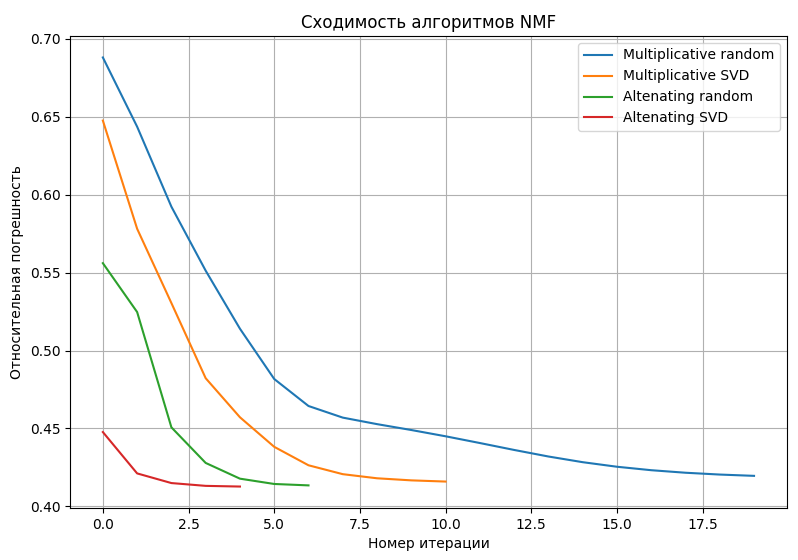
\includegraphics[width=\linewidth]{assets/Graph1.png}
  \caption{График относительной погрешности}
  \label{fig:relativeApproximationError}
\end{figure}

\newpage


Ниже приведены данные показывающие затраты по времени на выполнение алгоритмов:
\\

\begin{lstlisting}[caption=Затраты по времени на выполнение алгоритмов]
# Initialization:
Random takes 2.002e-05s
SVD takes 4.435e-04s
# Methods:
Multiplicative random takes 3.202e-03s
Multiplicative SVD takes 6.939e-04s
Altenating random takes 1.151e-02s
Altenating SVD takes 6.742e-03s
\end{lstlisting}

Ниже приведены результаты алгоритма попеременных наименьших квадратов с использованием SVD инициализации:

\begin{align*}
W H =
\begin{pmatrix}
     0.153  &   0  &   0.089 \\
     0  &   0  &   0.518 \\
     0  &   0  &   0.518 \\
     0.372  &   0.099  &   0 \\
     0.237  &   0  &   0 \\
     0  &   0.516  &   0 \\
     0.525  &  	0  &   0.027 \\
     0.042  &   0.752  &   0 \\
     0.229  &   0.131  &   0.613 \\
     0.042  &   0.752  &   0
\end{pmatrix}
\begin{pmatrix}
     2.152  &   0  &   1.897  &   1.530  &  0 \\
     0  &   1.472  &   1.022  &   0  &   0 \\
     0  &   0  &   0.250  &   0.493  &   1.844
\end{pmatrix}
\end{align*}



\newpage



Полученные данные можно интерпретировать в виде следующих таблиц:

\begin{center}
 \begin{tabular}{ l | c c c c c c }
 Термин      & 1 & 2 & 3 \\
 \hline
 eigenvalue  & 0.153  &   0  &   0.089 \\
 England     & 0  &   0  &   0.518 \\
 FIFA        & 0  &   0  &   0.518 \\
 Google      & 0.372  &   0.099  &   0 \\
 Internet    & 0.237  &   0  &   0 \\
 link        & 0  &   0.516  &   0 \\
 matrix      & 0.525  &  	0  &   0.027 \\
 page        & 0.042  &   0.752  &   0 \\
 rank        & 0.229  &   0.131  &   0.613 \\
 Web         & 0.042  &   0.752  &   0
\end{tabular}
\end{center}

\begin{center}
 \begin{tabular}{ l | c c c c c c }
 Вектор      & Док 1 & Док 2 & Док 3 & Док 4 & Док 5 \\
 \hline
 1           & 2.152  &   0  &   1.897  &   1.530  &  0 \\
 2           & 0  &   1.472  &   1.022  &   0  &   0 \\
 3           & 0  &   0  &   0.250  &   0.493  &   1.844 \\
\end{tabular}
\end{center}




\newpage





\section{Тестирование на разреженных данных}

Для тестирования алгоритмов на больших разреженных данных
построим разложение ранга $25$ с использованием терм-документной матрицы,
построенной на основе всех томов классического произведения \say{Война и Мир}.



\subsection{Результат}



\begin{tikzpicture}[
  trim axis left,
  every mark/.append style={mark size=4pt},
]
  \begin{axis}[
    axis lines = left,
    scale only axis,
    grid = major,
    title = График сходимости алгоритмов,
    xlabel = Номер итерации,
    ylabel = Ошибка,
    width = 0.9\textwidth,
    height = 0.7\textwidth,
    enlarge x limits={0.05},
    enlarge y limits={0.05},
    line width=1pt,
  ]

    \addplot table [
      x=iteration,
      y=roadside_picnic.5.ALS_LSQR,
      col sep=comma,
      skip coords between index={0}{1},
    ] {../samples/data.csv};
    \addlegendentry{ALS\_LSQR}

    \addplot table [
      x=iteration,
      y=roadside_picnic.5.ALS_NNLS,
      col sep=comma,
      skip coords between index={0}{1},
    ] {../samples/data.csv};
    \addlegendentry{ALS\_NNLS}

    \addplot table [
      x=iteration,
      y=roadside_picnic.5.ALS_NORM,
      col sep=comma,
      skip coords between index={0}{1},
    ] {../samples/data.csv};
    \addlegendentry{ALS\_NORM}

    \addplot table [
      x=iteration,
      y=roadside_picnic.5.MU,
      col sep=comma,
      skip coords between index={0}{1},
    ] {../samples/data.csv};
    \addlegendentry{MU}

  \end{axis}
\end{tikzpicture}

\newpage

Ниже приведены данные показывающие затраты по времени на выполнение алгоритмов:
\\

\begin{lstlisting}[caption=Затраты по времени на выполнение алгоритмов]
  ### Testing ###

  Parsing file war_and_peace.txt
  Rank 25

  # Generating weighted term-document matrix

  > Building term-count dictinaries
  [progress] took 14.87s, 53284 of 53284 done

  > Gathering all terms
  [progress] took 0.23s, 53284 of 53284 done

  > Merging frequency table
  [progress] took 76.55s, 53284 of 53284 done

  > Computing document-term frequency
  [progress] took 195.75s, 23306 of 23306 done

  > Generating weighted term-document matrix
  [progress] took 1.83s, 356551 of 356551 done

  Matrix a size (23306, 53284)


  # Iterations

  > Alternating least squares (solve)
  [progress] 16 steps, took 31.54s
  error 513.09485

  > Alternating least squares (nnls)
  [progress] 19 steps, took 40.52s
  error 514.91588

  > Alternating least squares (lstsq)
  [progress] 16 steps, took 68.34s
  error 513.09485

  > Multiplicative update rule
  [progress] 35 steps, took 67.10s
  error 513.50120

  Best - Alternating least squares (lstsq)
\end{lstlisting}




\newpage





\section{Тестирование на задачах интеллектуального анализа текста}

Для каждой рассмотренной задачи проведём выделение 5 ключевых предложений.
Анализ результата проведём в следующей секции.


\subsection{Результат метода оценки значимости}

\begin{itemize}
  \item И к бедным горбатым Больным верблюжатам, И каждого гоголем, Каждого моголем, Гоголем-моголем, Гоголем-моголем, Гоголем-моголем потчует
  \item И вывихнуто плечико У бедного кузнечика; Не прыгает, не скачет он, А горько-горько плачет он И доктора зовёт: О, где же добрый доктор
  \item И принесли к нему зайку, Такого больного, хромого, И доктор пришил ему ножки, И заинька прыгает снова
  \item Ах, жалко, жалко, жалко Бедных страусят
  \item Ах, у её малюток, У бедных акулят, Уже двенадцать суток Зубки болят
\end{itemize}



\subsection{Результат метода извлечение ключевых предложений из аппроксимации ранга $k$}

\begin{itemize}
  \item И к бедным горбатым Больным верблюжатам, И каждого гоголем, Каждого моголем, Гоголем-моголем, Гоголем-моголем, Гоголем-моголем потчует
  \item И вывихнуто плечико У бедного кузнечика; Не прыгает, не скачет он, А горько-горько плачет он И доктора зовёт: О, где же добрый доктор
  \item Десять ночей Айболит Не ест, не пьёт и не спит, Десять ночей подряд Он лечит несчастных зверят И ставит и ставит им градусники
  \item И бежит Айболит к бегемотикам, И хлопает их по животикам, И всем по порядку Даёт шоколадку, И ставит и ставит им градусники
  \item И горы встают перед ним на пути, И он по горам начинает ползти, А горы всё выше, а горы всё круче, А горы уходят под самые тучи
\end{itemize}




\newpage





\section{Выводы и комментарии}

\subsection{Тестирование на плотных данных малой размерности}

На Рис.~\ref{fig:relativeApproximationError} отчётливо видно,
что мультипликативным алогритмам необходимо в 2-3 раза больше итераций, чтобы добиться заданной точности.
Также график показывает, что мультипликативные алгоритмы чаще сходятся к более \say{плохой} точке локального минимума,
которая даёт меньшую точность разложения.
Касательно алгоритмов попеременных наименьших квадратов видно, что даже после первой итерации
относительная ошибка значительно меньше чем у предыдущих алгоритмов и в целом они требуют намного меньше итераций.

В обоих случаях инициализация матриц $W$ и $H$ с помощью сингулярного разложения понижает ошибку на первой итерации и уменьшает количество итерации.

Напомним, что первые четыре документа рассказывают о Google и рейтинге веб-страниц,
а пятый касается футбола. Из таблиц можно увидеть, что первые четыре документа представлены векторами,
которые имеют большие компоненты для ключевых слов, связанных с Google.
В отличие от этого, пятый документ представлен только третьим базисным вектором, так же с большой компонентой.
Мы видим, что третий вектор представляет документы рассказывающие о футболе, а два других показывают документы, связанные с Google.


\newpage


\subsection{Тестирование на разреженных данных}

Из графика видно, мультипликативные алгоритмы требуют намного больше итераций, чем альтернативы,
такие как алгоритмы попеременных наименьших квадратов, и работа на онду итерацию предельно высока.
Каждая итерация требует шесть $O(n^3)$ матрично-матричных умножений полностью плотных матриц и шесть
$O (n^2)$ покомпонентных операций.

Один недостаток мультипликативных алгоритмов состоит в том, что как только элемент в $W$ или $H$ становится 0,
он будет оставаться равным 0. Эта блокировка нулевых элементов означает, что,
как только алгоритм начинает двигаться по пути к фиксированной точке,
даже если это плохая фиксированная точка, он будет продолжать двигаться в том же направлении.

Алгоритмы ALS являются более гибкими, позволяя итеративному процессу уйти с неправильного пути.
В зависимости от реализации алгоритмы ALS могут быть достаточно быстрыми.



\newpage



\subsection{Тестирование на задачах интеллектуального анализа текста}

Метод, основанный на оценках значимости, имеет недостаток:
если в тексте присутсвуют два и более «самых значимых предложения», которые содержат одинаковые термы высокой значимости,
то их координаты будут примерно одинаковыми, и оба предложения будут извлечены как ключевые.
Но это не практично со стороны поиска информации, так как они очень похожи.

По результатам видно, что оба метода предпочитают более длинные предложения.

Также по результатам можно понять, что метод извлечение ключевых предложений из аппрок-
симации ранга $k$ старается включить в выборку предложения касающиеся \say{ортогональных} тем.
Под \say{ортогональностью} тем подразумевается их разнородность и в некотрой мере субъектиная оценка.
Такие свойства метода напрямую вытекают из использования $QR$ разложения.

Учитывая всё вышесказанное, можно сделать вывод, что метод извлечение ключевых предложений из
аппроксимации ранга $k$ даёт более качественную выборку, однако требует больше вычислительных ресурсов.
